% DOC SETTINGS ===================================
\documentclass{article}
\usepackage[utf8]{inputenc}
\usepackage{fancyhdr}
\pagestyle{fancy}
\usepackage{listings}
\usepackage{geometry}
 \geometry{
 a4paper,
 total={170mm,257mm},
 left=20mm,
 top=25mm,
 }
\fancyheadoffset{0mm}
\lhead{ECE2714 Problem Set 2}
\rhead{Kavin Thirukonda 2021}
\usepackage{steinmetz}
\usepackage{mathtools}  
\usepackage{multicol}
\usepackage{amsfonts}
\mathtoolsset{showonlyrefs} 
\cfoot{}
% DOC SETTINGS ===================================
\begin{document}
\begin{enumerate}
\item Plot the following DT signal in Python
\begin{equation}
    x[n] = \left(\frac{1}{5}\right)^{-n} u[-n] +\left(\frac{2}{3}\right)^nu[n]
\end{equation}  
Choose appropriate bounds to best highlight the behaviour of the signal and include your code.

\lstset{language=Python}
\lstset{frame=lines}
\lstset{label={lst:code_direct}}
\lstset{basicstyle=\footnotesize}
\begin{lstlisting}
    import numpy as np
    import matplotlib.pyplot as plt
    
    
    def x(n):
        return (1/5)**(-n)*np.heaviside(-n, 1) + (2/3)**n * np.heaviside(n, 1)
    
    
    n = np.linspace(-10, 10, 19)
    plt.stem(n, x(n))
    plt.show()
\end{lstlisting}
\begin{center}
    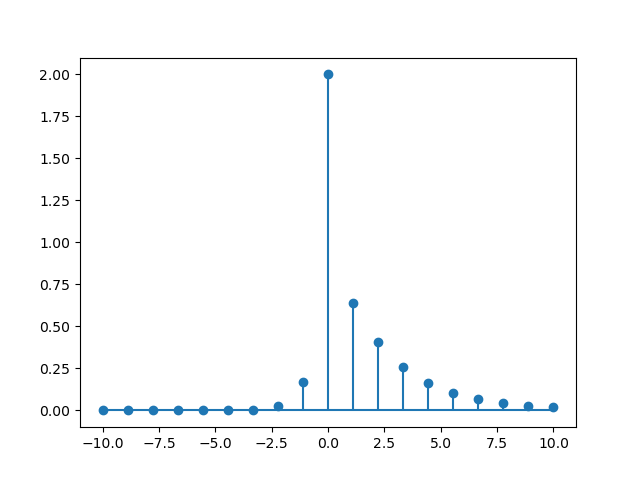
\includegraphics[width = .6\textwidth]{1.png}
\end{center}
\newpage
\item Solve the following differential equation
\begin{equation}
    \frac{d^2y}{dt^2}(t) + 4 \frac{dy}{dt}(t) + 13y(t) = 0
\end{equation}
using the auxiliary conditions $y(0) = 1$ and $\frac{dy}{dt}(0) = 1$.

Find general form:
\begin{align}
     \frac{d^2y}{dt^2}(t) + 4 \frac{dy}{dt}(t) + 13y(t) = 0 &\Rightarrow r^2 +4r +13 = 0\\
     &\Rightarrow r = \frac{-4 \pm \sqrt{4^2 -4(13)}}{2}\\
     &\Rightarrow r = \frac{-4 \pm \sqrt{-36}}{2}\\
     &\Rightarrow r = \frac{-4 \pm 6j}{2}\\
     &\Rightarrow r = -2 \pm 3j\\
     &\Rightarrow y = e^{-2t}\left(C_1\cos \left(3t\right)+C_2\sin \left(3t\right)\right)
\end{align}
$y(0) = 1$:    
\begin{align}
    1 &= \left(C_1\cos \left(0\right)+C_2\sin \left(0\right)\right)\\
    C_1 &= 1
\end{align}
$\frac{dy}{dt}(0) = 1$:    
\begin{align}
     y &= e^{-2t}(C_1\cos (3t)+C_2\sin(3t))\\
    \frac{d}{dt}(y) &= \frac{d}{dt}(e^{-2t}\left(C_1\cos \left(3t\right)+C_2\sin \left(3t\right)\right)\\
    \frac{dy}{dt} &= -2e^{-2x}\left(C_1\cos \left(3t\right)+C_2\sin \left(3t\right)\right)+e^{-2t}\left(-3C_1\sin \left(3t\right)+ 3C_2\cos \left(3t\right)\right)\\
    1 &= -2e^0(\cos(0)+C_2\sin(0))+e^0(-3\sin(0)+3C_2\cos(0))\\
    C_2 &= 1
\end{align}

\begin{equation}
    \boxed{y = e^{-2t}\left(\cos \left(3t\right)+\sin \left(3t\right)\right)}
\end{equation}
\newpage
\item Find the impulse response of the following system
\begin{equation}
    \frac{d^2y}{dt^2}(t) + 4\frac{dy}{dt}(t) + 13y(t) = - \frac{dx}{dt}(t) + 2x(t) 
\end{equation}
\begin{center}
    we can redefine the system as:
\end{center}
\begin{equation}
    D^2y(t)+4D^1y(t)+13y(t)= -D^1x(t)+2x(t)
\end{equation}
\begin{center}
    Because $N > M$ the impulse response of the system is (Using initial conditions y''(0) = 1 $\&$ $y^{(k)}(0) = 0$):
\end{center}
\begin{equation}
    h(t) = \left(\frac{dy_h(t)}{dt}+ 2y_h(t)\right)u(t)
\end{equation}
$y(0) = 0$:    
\begin{align}
    1 &= \left(C_1\cos \left(0\right)+C_2\sin \left(0\right)\right)\\
    C_2 &= 1
\end{align}
$y''(0) = 1$:    
\begin{align}
     y &= e^{-2t}(C_1\cos (3t)+C_2\sin(3t))\\
    \frac{d}{dt}(y) &= \frac{d}{dt}(e^{-2t}\left(C_1\cos \left(3t\right)+C_2\sin \left(3t\right)\right)\\
    y' &= -2e^{-2x}\left(C_1\cos \left(3t\right)+C_2\sin \left(3t\right)\right)+e^{-2t}\left(-3C_1\sin \left(3t\right)+ 3C_2\cos \left(3t\right)\right)\\
    \frac{d}{dt}(y') &= \frac{d}{dt}(-2e^{-2x}\left(C_1\cos \left(3t\right)+C_2\sin \left(3t\right)\right)+e^{-2t}\left(-3C_1\sin \left(3t\right)+ 3C_2\cos \left(3t\right)\right))\\
    y'' &= 4e^{-2x}\left(C_1\cos \left(3t\right)+C_2\sin \left(3t\right)\right)\\
    1 &= 4e^{0}\left(C_1\cos \left(0\right)+(1)\sin \left(0\right)\right)\\
    1 &= 4\left(C_1\right)\\
    C_1 = \frac{1}{4}
\end{align}
\begin{center}
    using all this information we can find the homogeneous solution and use that to find the complete impulse response:
\end{center}
\begin{equation}
    y_h = e^{-2t}\left(\frac{1}{4}\cos(3t)+\sin(3t)\right)
\end{equation}
\begin{equation}
    \boxed{h(t) = \left(\frac{d}{dt}\left(e^{-2t}\left(\frac{1}{4}\cos(3t)+\sin(3t)\right)\right)+ 2\left(e^{-2t}\left(\frac{1}{4}\cos(3t)+\sin(3t)\right)\right)\right)u(t)}
\end{equation}
\newpage
\item Consider $x[n] = e^{\frac{j12\pi}{21}n}\{u[n] - u[n - 10]\}$.

\lstset{language=Python}
\lstset{frame=lines}
\lstset{label={lst:code_direct}}
\lstset{basicstyle=\footnotesize}
\begin{lstlisting}
    import numpy as np
    import matplotlib.pyplot as plt
    
    
    def x(n):
        return np.e**((12j*np.pi*n)/21)*(np.heaviside(n, 1)-np.heaviside(n-10, 1))
    
    
    n = np.arange(-5, 15, 1)
    plt.stem(n, abs(x(n)), basefmt="C0-")
    plt.title("Magnitude")
    plt.show()
    plt.stem(n, np.angle(x(n)), basefmt="C0-")
    plt.title("Phase")
    plt.show()
    plt.stem(n, abs(x(2*n)), basefmt="C0-")
    plt.title("Magnitude")
    plt.show()
    plt.stem(n, np.angle(x(n)), basefmt="C0-")
    plt.title("Phase")
    plt.show()
    n = np.arange(-5, 25, 1)
    plt.stem(n, abs(x(n/2)), basefmt="C0-")
    plt.title("Magnitude")
    plt.show()
    plt.stem(n, np.angle(x(n)), basefmt="C0-")
    plt.title("Phase")
    plt.show()
\end{lstlisting}
\begin{enumerate}
    \item Plot $\lvert x[n] \lvert$ and $\phase{x[n]}$ for $-5 \leq n \leq 15.$
    \begin{center}
        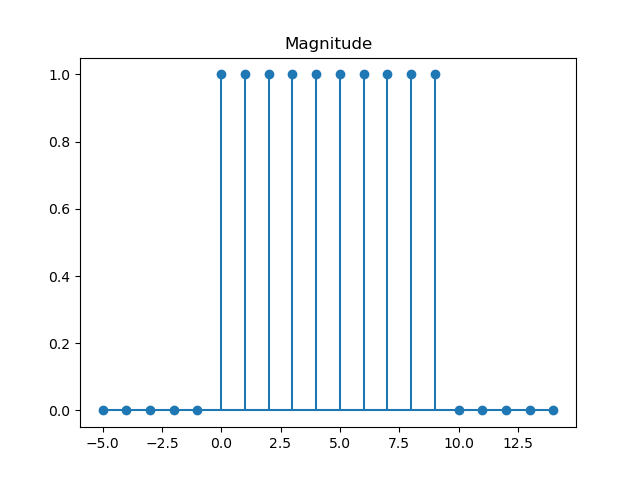
\includegraphics[width = .3375\textwidth]{4a1.png}
        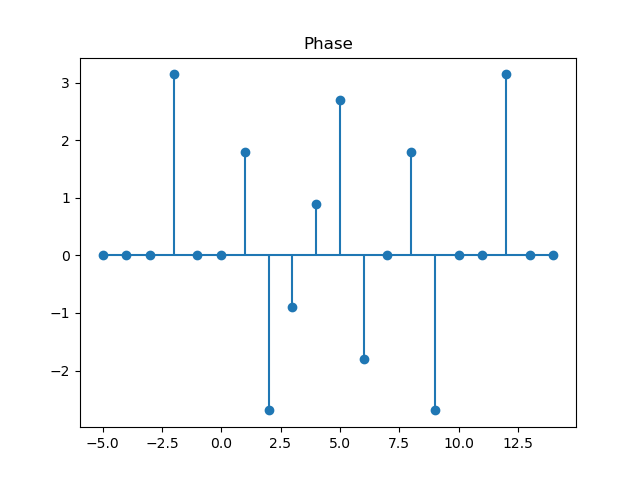
\includegraphics[width = .3375\textwidth]{4a2.png}
    \end{center}
    \item Plot the magnitude and phase of the decimated signal $y[n] = x[2n]$ for $-5 \leq n \leq 15.$
    \begin{center}
        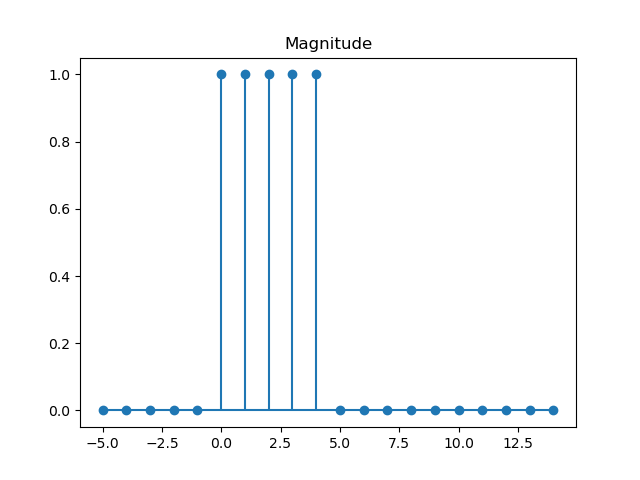
\includegraphics[width = .3375\textwidth]{4b1.png}
        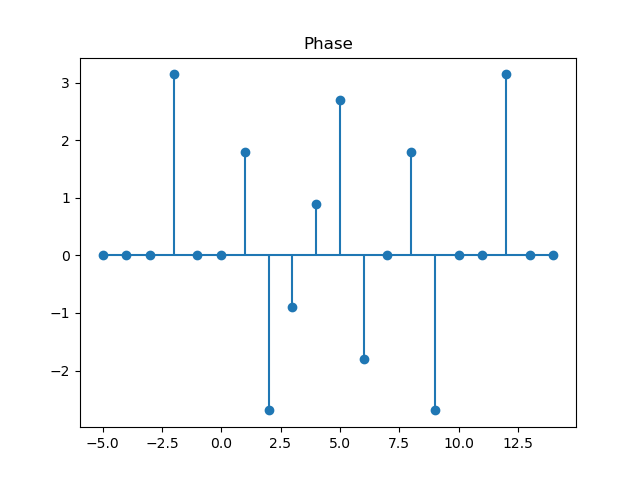
\includegraphics[width = .3375\textwidth]{4b2.png}
    \end{center}
    \item Plot the magnitude and phase of the interpolated signal $y[n] = x[\frac{n}{2}]$ for $-5 \leq n \leq 25.$
    \begin{center}
        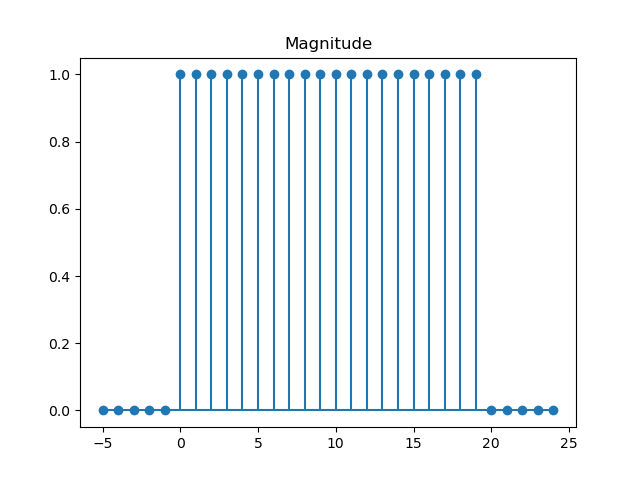
\includegraphics[width = .3375\textwidth]{4c1.png}
        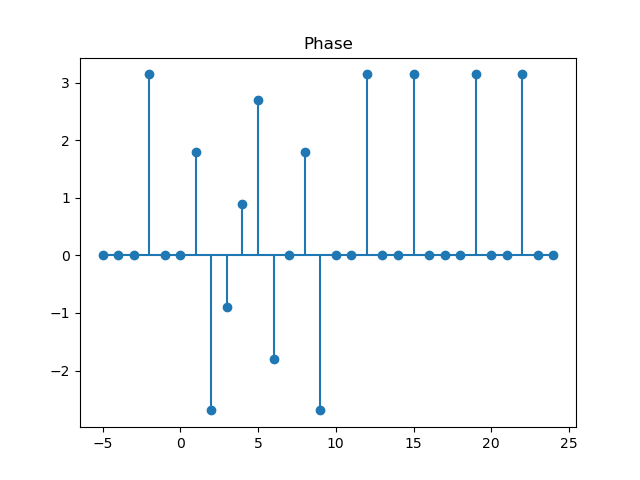
\includegraphics[width = .3375\textwidth]{4c2.png}
    \end{center}
\end{enumerate}
\newpage
\item Consider the signal $x[n] = e^{j\frac{10\pi}{7}n}$.
\begin{enumerate}
    \item Is this signal periodic? If so, what is the period?
    \begin{center}
        Yes the signal is \boxed{periodic}, with a period of \boxed{5}.
    \end{center}
    \item Calculate the power and energy of this signal.
    \begin{enumerate}
        \item Power
        \begin{equation}
            \lim_{n\rightarrow\infty}\frac{1}{2N+1}\sum_{-N}^{N}\lvert e^{j\frac{10\pi}{7}n}\lvert^2 = \boxed{\infty}
        \end{equation}
        \item Energy
        \begin{equation}
            \sum_{-\infty}^{\infty}\lvert e^{j\frac{10\pi}{7}n}\lvert^2 = \boxed{1}
        \end{equation}
    \end{enumerate}
    \item is $\Re (x[n])$ even, odd or neither?
    \begin{center}
        \boxed{Even}
    \end{center}
    \item is $\Im(x[n])$ even, odd or neither?
    \begin{center}
        \boxed{Odd}
    \end{center}
    \item Consider $y[n] = e^{j\frac{24\pi}{7}n}$. Does $x[n] = y[n]$? How do you know?
    \begin{center} 
        \boxed{Yes}, because y[n] is a "shift" of $2\pi$ to the angle which results in the same function.
    \end{center}
    \item Consider $y[n] = e^{j\frac{16\pi}{7}n}$. Does $x[n] = y[n]$? How do you know?
    \begin{center} 
        \boxed{No}, because y[n] cannot be represented as a "shift" of $2\pi$ to the angle.
    \end{center}
    \item Let $z[n] = \frac{x[n]}{y[n]}$ where $y[n] = e^{j\frac{5}{3}n}$. Is z[n] periodic? how do you know?
    \begin{equation}
        z[n] = \frac{e^{j\frac{5}{3}n}}{e^{j\frac{5}{3}n}} 
    \end{equation}
    \begin{center}
        By subtracting exponents and solving we can clearly see that the signal is not a rational multiple of 2$\pi$ and therefore is \boxed{aperiodic}
    \end{center}
\end{enumerate} 
\newpage
\item Consider the periodic discrete-time exponential time signal given by the expression,
\begin{equation}
    x[n] = e^{jm\frac{2\pi}{N}n}.
\end{equation}
Show that the fundamental period of this signal is given by the expression,
\begin{equation}
    N_0 = \frac{N}{gcd(m,N)},
\end{equation}
Where gcd(m,N) is the greatest common divisor of m and N; that is, the largest integer that divides both m and N an integral number of times. For example,
\begin{align}
    gcd(2,3) &= 1,\\
    gcd(2,4) &= 2,\\
    gcd(8,12) &= 4,
\end{align}
Note that $N_0 = N$ if m and N have no factors in common.
\begin{align}
    e^{jm\frac{2\pi}{N}n} &= e^{j2\pi k}\\
    m\frac{2\pi}{N}n &= 2\pi k\\
    N_0 = \frac{N}{(m/k)}
\end{align}
\begin{center}
    Therefore the following statement is true:
\end{center}
\begin{equation}
    N_0 = \frac{N}{gcd(m,N)},
\end{equation}
\newpage
\item Let x(t) be the continuous-time complex exponential signal given by the expression,
\begin{equation}
    x(t) = e^{j\omega_0t}
\end{equation}
with the fundamental frequency $\omega_0$ and the fundamental period
\begin{equation}
    T_0 = \frac{2\pi}{\omega_0}.
\end{equation}
Consider the discrete-time signal obtained by taking equally spaced samples of x(t) such that 
\begin{align}
    x[n] &= x(nT),\\
    &= e^{j\omega_0nT}.
\end{align}
Show that x[n] is periodic if and only if $\frac{T}{T_0}$ if a rational number; that is, if and only if some multiple of the sampling interval exactly equals a multiple of the period of x(t).
\begin{center}
    if x[n] is periodic then any rational multiple of $2\pi$ factored into the exponent would result in the same function. This means that:
\end{center}
\begin{equation}
    \frac{T}{T_0} = \frac{k}{N} = \mathbb{Q}
\end{equation}
\begin{center}
    That is the closest thing to a proof that I can conjure.
\end{center}
\newpage
\end{enumerate}
\end{document}
